% Options for packages loaded elsewhere
\PassOptionsToPackage{unicode}{hyperref}
\PassOptionsToPackage{hyphens}{url}
\PassOptionsToPackage{dvipsnames,svgnames,x11names}{xcolor}
%
\documentclass[
]{article}
\usepackage{amsmath,amssymb}
\usepackage{lmodern}
\usepackage{iftex}
\ifPDFTeX
  \usepackage[T1]{fontenc}
  \usepackage[utf8]{inputenc}
  \usepackage{textcomp} % provide euro and other symbols
\else % if luatex or xetex
  \usepackage{unicode-math}
  \defaultfontfeatures{Scale=MatchLowercase}
  \defaultfontfeatures[\rmfamily]{Ligatures=TeX,Scale=1}
\fi
% Use upquote if available, for straight quotes in verbatim environments
\IfFileExists{upquote.sty}{\usepackage{upquote}}{}
\IfFileExists{microtype.sty}{% use microtype if available
  \usepackage[]{microtype}
  \UseMicrotypeSet[protrusion]{basicmath} % disable protrusion for tt fonts
}{}
\makeatletter
\@ifundefined{KOMAClassName}{% if non-KOMA class
  \IfFileExists{parskip.sty}{%
    \usepackage{parskip}
  }{% else
    \setlength{\parindent}{0pt}
    \setlength{\parskip}{6pt plus 2pt minus 1pt}}
}{% if KOMA class
  \KOMAoptions{parskip=half}}
\makeatother
\usepackage{xcolor}
\usepackage[margin=1in]{geometry}
\usepackage{color}
\usepackage{fancyvrb}
\newcommand{\VerbBar}{|}
\newcommand{\VERB}{\Verb[commandchars=\\\{\}]}
\DefineVerbatimEnvironment{Highlighting}{Verbatim}{commandchars=\\\{\}}
% Add ',fontsize=\small' for more characters per line
\usepackage{framed}
\definecolor{shadecolor}{RGB}{248,248,248}
\newenvironment{Shaded}{\begin{snugshade}}{\end{snugshade}}
\newcommand{\AlertTok}[1]{\textcolor[rgb]{0.94,0.16,0.16}{#1}}
\newcommand{\AnnotationTok}[1]{\textcolor[rgb]{0.56,0.35,0.01}{\textbf{\textit{#1}}}}
\newcommand{\AttributeTok}[1]{\textcolor[rgb]{0.77,0.63,0.00}{#1}}
\newcommand{\BaseNTok}[1]{\textcolor[rgb]{0.00,0.00,0.81}{#1}}
\newcommand{\BuiltInTok}[1]{#1}
\newcommand{\CharTok}[1]{\textcolor[rgb]{0.31,0.60,0.02}{#1}}
\newcommand{\CommentTok}[1]{\textcolor[rgb]{0.56,0.35,0.01}{\textit{#1}}}
\newcommand{\CommentVarTok}[1]{\textcolor[rgb]{0.56,0.35,0.01}{\textbf{\textit{#1}}}}
\newcommand{\ConstantTok}[1]{\textcolor[rgb]{0.00,0.00,0.00}{#1}}
\newcommand{\ControlFlowTok}[1]{\textcolor[rgb]{0.13,0.29,0.53}{\textbf{#1}}}
\newcommand{\DataTypeTok}[1]{\textcolor[rgb]{0.13,0.29,0.53}{#1}}
\newcommand{\DecValTok}[1]{\textcolor[rgb]{0.00,0.00,0.81}{#1}}
\newcommand{\DocumentationTok}[1]{\textcolor[rgb]{0.56,0.35,0.01}{\textbf{\textit{#1}}}}
\newcommand{\ErrorTok}[1]{\textcolor[rgb]{0.64,0.00,0.00}{\textbf{#1}}}
\newcommand{\ExtensionTok}[1]{#1}
\newcommand{\FloatTok}[1]{\textcolor[rgb]{0.00,0.00,0.81}{#1}}
\newcommand{\FunctionTok}[1]{\textcolor[rgb]{0.00,0.00,0.00}{#1}}
\newcommand{\ImportTok}[1]{#1}
\newcommand{\InformationTok}[1]{\textcolor[rgb]{0.56,0.35,0.01}{\textbf{\textit{#1}}}}
\newcommand{\KeywordTok}[1]{\textcolor[rgb]{0.13,0.29,0.53}{\textbf{#1}}}
\newcommand{\NormalTok}[1]{#1}
\newcommand{\OperatorTok}[1]{\textcolor[rgb]{0.81,0.36,0.00}{\textbf{#1}}}
\newcommand{\OtherTok}[1]{\textcolor[rgb]{0.56,0.35,0.01}{#1}}
\newcommand{\PreprocessorTok}[1]{\textcolor[rgb]{0.56,0.35,0.01}{\textit{#1}}}
\newcommand{\RegionMarkerTok}[1]{#1}
\newcommand{\SpecialCharTok}[1]{\textcolor[rgb]{0.00,0.00,0.00}{#1}}
\newcommand{\SpecialStringTok}[1]{\textcolor[rgb]{0.31,0.60,0.02}{#1}}
\newcommand{\StringTok}[1]{\textcolor[rgb]{0.31,0.60,0.02}{#1}}
\newcommand{\VariableTok}[1]{\textcolor[rgb]{0.00,0.00,0.00}{#1}}
\newcommand{\VerbatimStringTok}[1]{\textcolor[rgb]{0.31,0.60,0.02}{#1}}
\newcommand{\WarningTok}[1]{\textcolor[rgb]{0.56,0.35,0.01}{\textbf{\textit{#1}}}}
\usepackage{longtable,booktabs,array}
\usepackage{calc} % for calculating minipage widths
% Correct order of tables after \paragraph or \subparagraph
\usepackage{etoolbox}
\makeatletter
\patchcmd\longtable{\par}{\if@noskipsec\mbox{}\fi\par}{}{}
\makeatother
% Allow footnotes in longtable head/foot
\IfFileExists{footnotehyper.sty}{\usepackage{footnotehyper}}{\usepackage{footnote}}
\makesavenoteenv{longtable}
\usepackage{graphicx}
\makeatletter
\def\maxwidth{\ifdim\Gin@nat@width>\linewidth\linewidth\else\Gin@nat@width\fi}
\def\maxheight{\ifdim\Gin@nat@height>\textheight\textheight\else\Gin@nat@height\fi}
\makeatother
% Scale images if necessary, so that they will not overflow the page
% margins by default, and it is still possible to overwrite the defaults
% using explicit options in \includegraphics[width, height, ...]{}
\setkeys{Gin}{width=\maxwidth,height=\maxheight,keepaspectratio}
% Set default figure placement to htbp
\makeatletter
\def\fps@figure{htbp}
\makeatother
\setlength{\emergencystretch}{3em} % prevent overfull lines
\providecommand{\tightlist}{%
  \setlength{\itemsep}{0pt}\setlength{\parskip}{0pt}}
\setcounter{secnumdepth}{-\maxdimen} % remove section numbering
\usepackage[width=0.8\textwidth]{caption}
\ifLuaTeX
  \usepackage{selnolig}  % disable illegal ligatures
\fi
\IfFileExists{bookmark.sty}{\usepackage{bookmark}}{\usepackage{hyperref}}
\IfFileExists{xurl.sty}{\usepackage{xurl}}{} % add URL line breaks if available
\urlstyle{same} % disable monospaced font for URLs
\hypersetup{
  pdftitle={Title},
  pdfauthor={Christian Oppegård Moen},
  colorlinks=true,
  linkcolor={Maroon},
  filecolor={Maroon},
  citecolor={Blue},
  urlcolor={blue},
  pdfcreator={LaTeX via pandoc}}

\title{Title}
\usepackage{etoolbox}
\makeatletter
\providecommand{\subtitle}[1]{% add subtitle to \maketitle
  \apptocmd{\@title}{\par {\large #1 \par}}{}{}
}
\makeatother
\subtitle{Course}
\author{Christian Oppegård Moen}
\date{DD MM YYYY}

\begin{document}
\maketitle

{
\hypersetup{linkcolor=}
\setcounter{tocdepth}{3}
\tableofcontents
}
\hypertarget{libraries}{%
\section{Libraries}\label{libraries}}

\begin{Shaded}
\begin{Highlighting}[]
\FunctionTok{library}\NormalTok{(glmm)}
\FunctionTok{library}\NormalTok{(dplyr)}
\end{Highlighting}
\end{Shaded}

\hypertarget{data}{%
\section{Data}\label{data}}

Data format is of tab separated values regarding noise on campus. Some variables are shown in the printout below. The response is \texttt{spmTriv} and \texttt{spmEff} which are ``trivsel'' and ``effektivitet'', respectively. The response is evaluated for each building block.

\hypertarget{load-data-and-reformat}{%
\subsection{Load data and reformat}\label{load-data-and-reformat}}

\begin{Shaded}
\begin{Highlighting}[]
\NormalTok{pathData }\OtherTok{=} \StringTok{"./data"}
\NormalTok{d }\OtherTok{=} \FunctionTok{read.delim}\NormalTok{(}\StringTok{"./data/data{-}315297{-}2023{-}03{-}08{-}1434{-}utf.txt"}\NormalTok{, }\AttributeTok{header =}\NormalTok{ T)}

\CommentTok{\# Reformat the time to be total time in seconds}
\NormalTok{formatTime }\OtherTok{\textless{}{-}} \ControlFlowTok{function}\NormalTok{(t) \{}
\NormalTok{    tSplit }\OtherTok{=} \FunctionTok{strsplit}\NormalTok{(t, }\StringTok{" "}\NormalTok{)[[}\DecValTok{1}\NormalTok{]]}
\NormalTok{    s }\OtherTok{=} \DecValTok{0}
    \ControlFlowTok{for}\NormalTok{ (i }\ControlFlowTok{in} \FunctionTok{seq}\NormalTok{(}\DecValTok{1}\NormalTok{, }\FunctionTok{length}\NormalTok{(tSplit), }\DecValTok{2}\NormalTok{)) \{}
\NormalTok{        s }\OtherTok{=}\NormalTok{ s }\SpecialCharTok{+} \ControlFlowTok{switch}\NormalTok{(tSplit[i }\SpecialCharTok{+} \DecValTok{1}\NormalTok{], }\AttributeTok{dag =} \FunctionTok{strtoi}\NormalTok{(tSplit[i]) }\SpecialCharTok{*} \DecValTok{24} \SpecialCharTok{*} \DecValTok{3600}\NormalTok{, }\AttributeTok{dager =} \FunctionTok{strtoi}\NormalTok{(tSplit[i]) }\SpecialCharTok{*}
            \DecValTok{24} \SpecialCharTok{*} \DecValTok{3600}\NormalTok{, }\AttributeTok{time =} \FunctionTok{strtoi}\NormalTok{(tSplit[i]) }\SpecialCharTok{*} \DecValTok{3600}\NormalTok{, }\AttributeTok{timer =} \FunctionTok{strtoi}\NormalTok{(tSplit[i]) }\SpecialCharTok{*}
            \DecValTok{3600}\NormalTok{, }\AttributeTok{minutt =} \FunctionTok{strtoi}\NormalTok{(tSplit[i]) }\SpecialCharTok{*} \DecValTok{60}\NormalTok{, }\AttributeTok{minutter =} \FunctionTok{strtoi}\NormalTok{(tSplit[i]) }\SpecialCharTok{*}
            \DecValTok{60}\NormalTok{, }\AttributeTok{sekund =} \FunctionTok{strtoi}\NormalTok{(tSplit[i]), }\AttributeTok{sekunder =} \FunctionTok{strtoi}\NormalTok{(tSplit[i]), }\DecValTok{0}\NormalTok{)}
\NormalTok{    \}}
    \FunctionTok{return}\NormalTok{(s)}
\NormalTok{\}}

\NormalTok{ftimes }\OtherTok{=} \FunctionTok{unlist}\NormalTok{(}\FunctionTok{lapply}\NormalTok{(d}\SpecialCharTok{$}\NormalTok{Svartid, formatTime))}
\FunctionTok{head}\NormalTok{(}\FunctionTok{cbind}\NormalTok{(}\AttributeTok{old =}\NormalTok{ d}\SpecialCharTok{$}\NormalTok{Svartid, }\AttributeTok{new =}\NormalTok{ ftimes))}
\end{Highlighting}
\end{Shaded}

\begin{verbatim}
##      old                      new  
## [1,] "2 minutter 32 sekunder" "152"
## [2,] "1 minutt 58 sekunder"   "118"
## [3,] "2 minutter 32 sekunder" "152"
## [4,] "4 minutter 28 sekunder" "268"
## [5,] "2 minutter 45 sekunder" "165"
## [6,] "2 minutter 41 sekunder" "161"
\end{verbatim}

\begin{Shaded}
\begin{Highlighting}[]
\NormalTok{d}\SpecialCharTok{$}\NormalTok{Svartid }\OtherTok{=}\NormalTok{ ftimes}
\end{Highlighting}
\end{Shaded}

\begin{Shaded}
\begin{Highlighting}[]
\FunctionTok{write.csv}\NormalTok{(d[d[, }\StringTok{"spmTekst"}\NormalTok{] }\SpecialCharTok{!=} \StringTok{""}\NormalTok{, }\FunctionTok{c}\NormalTok{(}\StringTok{"NR"}\NormalTok{, }\StringTok{"spmTekst"}\NormalTok{)], }\StringTok{"./data/freeTxt.csv"}\NormalTok{, }\AttributeTok{row.names =} \ConstantTok{FALSE}\NormalTok{)}
\end{Highlighting}
\end{Shaded}

\begin{Shaded}
\begin{Highlighting}[]
\NormalTok{N }\OtherTok{=} \FunctionTok{length}\NormalTok{(d[, }\DecValTok{1}\NormalTok{])}
\NormalTok{ancPercentage }\OtherTok{=} \FunctionTok{length}\NormalTok{(d}\SpecialCharTok{$}\NormalTok{spmTiltak\_1[d}\SpecialCharTok{$}\NormalTok{spmTiltak\_1 }\SpecialCharTok{==} \StringTok{"mNc"}\NormalTok{])}\SpecialCharTok{/}\NormalTok{N}
\NormalTok{ancPercentage}
\end{Highlighting}
\end{Shaded}

\begin{verbatim}
## [1] 0.7686567
\end{verbatim}

\hypertarget{response-empirical-mean-and-standard-deviations-sd}{%
\subsection{Response (empirical mean and standard deviations (SD))}\label{response-empirical-mean-and-standard-deviations-sd}}

Compute per building means and SDs

\begin{Shaded}
\begin{Highlighting}[]
\CommentTok{\# All locations/buildings}
\NormalTok{locs }\OtherTok{=} \FunctionTok{unique}\NormalTok{(d}\SpecialCharTok{$}\NormalTok{spmHvor)}

\CommentTok{\# initiate per building empirical mean data frame}
\NormalTok{buildMeans }\OtherTok{=} \FunctionTok{data.frame}\NormalTok{(}\FunctionTok{matrix}\NormalTok{(}\AttributeTok{ncol =} \FunctionTok{length}\NormalTok{(locs), }\AttributeTok{nrow =} \DecValTok{2}\NormalTok{, }\AttributeTok{dimnames =} \FunctionTok{list}\NormalTok{(}\FunctionTok{c}\NormalTok{(}\StringTok{"trivsel"}\NormalTok{,}
    \StringTok{"effektivitet"}\NormalTok{), locs)))}
\CommentTok{\# initiate per building standard deviation data frame}
\NormalTok{buildSd }\OtherTok{=} \FunctionTok{data.frame}\NormalTok{(}\FunctionTok{matrix}\NormalTok{(}\AttributeTok{ncol =} \FunctionTok{length}\NormalTok{(locs), }\AttributeTok{nrow =} \DecValTok{2}\NormalTok{, }\AttributeTok{dimnames =} \FunctionTok{list}\NormalTok{(}\FunctionTok{c}\NormalTok{(}\StringTok{"trivsel"}\NormalTok{,}
    \StringTok{"effektivitet"}\NormalTok{), locs)))}
\CommentTok{\# Compute means and SDs}
\ControlFlowTok{for}\NormalTok{ (loc }\ControlFlowTok{in}\NormalTok{ locs) \{}
\NormalTok{    buildMeans[loc] }\OtherTok{=} \FunctionTok{c}\NormalTok{(}\FunctionTok{mean}\NormalTok{(d}\SpecialCharTok{$}\NormalTok{spmTriv[d}\SpecialCharTok{$}\NormalTok{spmHvor }\SpecialCharTok{==}\NormalTok{ loc]), }\FunctionTok{mean}\NormalTok{(d}\SpecialCharTok{$}\NormalTok{spmEff[d}\SpecialCharTok{$}\NormalTok{spmHvor }\SpecialCharTok{==}
\NormalTok{        loc]))}
\NormalTok{    buildSd[loc] }\OtherTok{=} \FunctionTok{c}\NormalTok{(}\FunctionTok{sd}\NormalTok{(d}\SpecialCharTok{$}\NormalTok{spmTriv[d}\SpecialCharTok{$}\NormalTok{spmHvor }\SpecialCharTok{==}\NormalTok{ loc]), }\FunctionTok{sd}\NormalTok{(d}\SpecialCharTok{$}\NormalTok{spmEff[d}\SpecialCharTok{$}\NormalTok{spmHvor }\SpecialCharTok{==}\NormalTok{ loc]))}
\NormalTok{\}}
\NormalTok{buildMeans[}\DecValTok{1}\SpecialCharTok{:}\DecValTok{5}\NormalTok{]}
\end{Highlighting}
\end{Shaded}

\begin{verbatim}
##               elD      elB     kjel  elE     real
## trivsel      3.75 3.714286 3.666667 4.35 2.600000
## effektivitet 3.50 3.857143 3.000000 3.95 2.666667
\end{verbatim}

\begin{Shaded}
\begin{Highlighting}[]
\NormalTok{buildSd[}\DecValTok{1}\SpecialCharTok{:}\DecValTok{5}\NormalTok{]}
\end{Highlighting}
\end{Shaded}

\begin{verbatim}
##              elD       elB     kjel       elE     real
## trivsel      0.5 0.7559289 1.751190 0.8127277 1.328728
## effektivitet 1.0 1.2149858 1.414214 1.0990426 1.321789
\end{verbatim}

\begin{Shaded}
\begin{Highlighting}[]
\FunctionTok{rbind}\NormalTok{(buildMeans, buildSd)[}\DecValTok{1}\SpecialCharTok{:}\DecValTok{5}\NormalTok{]}
\end{Highlighting}
\end{Shaded}

\begin{verbatim}
##                elD       elB     kjel       elE     real
## trivsel       3.75 3.7142857 3.666667 4.3500000 2.600000
## effektivitet  3.50 3.8571429 3.000000 3.9500000 2.666667
## trivsel1      0.50 0.7559289 1.751190 0.8127277 1.328728
## effektivitet1 1.00 1.2149858 1.414214 1.0990426 1.321789
\end{verbatim}

\begin{Shaded}
\begin{Highlighting}[]
\CommentTok{\# means}
\FunctionTok{write.table}\NormalTok{(}\FunctionTok{t}\NormalTok{(buildMeans[}\StringTok{"trivsel"}\NormalTok{, ]), }\AttributeTok{file =} \FunctionTok{paste}\NormalTok{(pathData, }\StringTok{"/trivselPerBygning.dat"}\NormalTok{,}
    \AttributeTok{sep =} \StringTok{""}\NormalTok{), }\AttributeTok{row.names =}\NormalTok{ T, }\AttributeTok{sep =} \StringTok{","}\NormalTok{, }\AttributeTok{quote =}\NormalTok{ F)}
\FunctionTok{write.table}\NormalTok{(}\FunctionTok{t}\NormalTok{(buildMeans[}\StringTok{"effektivitet"}\NormalTok{, ]), }\AttributeTok{file =} \FunctionTok{paste}\NormalTok{(pathData, }\StringTok{"/effektivitetPerBygning.dat"}\NormalTok{,}
    \AttributeTok{sep =} \StringTok{""}\NormalTok{), }\AttributeTok{row.names =}\NormalTok{ T, }\AttributeTok{sep =} \StringTok{","}\NormalTok{, }\AttributeTok{quote =}\NormalTok{ F)}
\CommentTok{\# Standard deviations (sd)}
\FunctionTok{write.table}\NormalTok{(}\FunctionTok{t}\NormalTok{(buildSd[}\StringTok{"trivsel"}\NormalTok{, ]), }\AttributeTok{file =} \FunctionTok{paste}\NormalTok{(pathData, }\StringTok{"/trivselPerBygningSD.dat"}\NormalTok{,}
    \AttributeTok{sep =} \StringTok{""}\NormalTok{), }\AttributeTok{row.names =}\NormalTok{ T, }\AttributeTok{sep =} \StringTok{","}\NormalTok{, }\AttributeTok{quote =}\NormalTok{ F)}
\FunctionTok{write.table}\NormalTok{(}\FunctionTok{t}\NormalTok{(buildSd[}\StringTok{"effektivitet"}\NormalTok{, ]), }\AttributeTok{file =} \FunctionTok{paste}\NormalTok{(pathData, }\StringTok{"/effektivitetPerBygningSD.dat"}\NormalTok{,}
    \AttributeTok{sep =} \StringTok{""}\NormalTok{), }\AttributeTok{row.names =}\NormalTok{ T, }\AttributeTok{sep =} \StringTok{","}\NormalTok{, }\AttributeTok{quote =}\NormalTok{ F)}
\end{Highlighting}
\end{Shaded}

\begin{Shaded}
\begin{Highlighting}[]
\CommentTok{\# æ is \textbackslash{}u00E6}
\CommentTok{\# ø is \textbackslash{}u00F8}
\CommentTok{\# å is \textbackslash{}u00E5}
\FunctionTok{barplot}\NormalTok{(}
\NormalTok{  ((}\FunctionTok{as.matrix}\NormalTok{(buildMeans))), }
  \AttributeTok{col =} \FunctionTok{c}\NormalTok{(}\StringTok{"lightblue"}\NormalTok{, }\StringTok{\textquotesingle{}darkblue\textquotesingle{}}\NormalTok{),}
  \AttributeTok{border =} \StringTok{"white"}\NormalTok{,}
  \CommentTok{\# main="Trivsel",}
  \AttributeTok{ylab=}\StringTok{"P\textbackslash{}u00E5virkning"}\NormalTok{,}
  \AttributeTok{beside =}\NormalTok{ T,}
  \AttributeTok{las=}\DecValTok{2}\NormalTok{,}
  \AttributeTok{ylim =} \FunctionTok{c}\NormalTok{(}\DecValTok{0}\NormalTok{,}\DecValTok{5}\NormalTok{)}
  \CommentTok{\# space=0.1}
\NormalTok{)}
\FunctionTok{legend}\NormalTok{(}
  \StringTok{"top"}\NormalTok{,}
  \AttributeTok{legend =} \FunctionTok{c}\NormalTok{(}\StringTok{"Trivsel"}\NormalTok{, }\StringTok{"Effektivitet"}\NormalTok{),}
  \AttributeTok{fill =} \FunctionTok{c}\NormalTok{(}\StringTok{"lightblue"}\NormalTok{, }\StringTok{\textquotesingle{}darkblue\textquotesingle{}}\NormalTok{), }\AttributeTok{bty =} \StringTok{\textquotesingle{}n\textquotesingle{}}\NormalTok{)}
\end{Highlighting}
\end{Shaded}

\begin{center}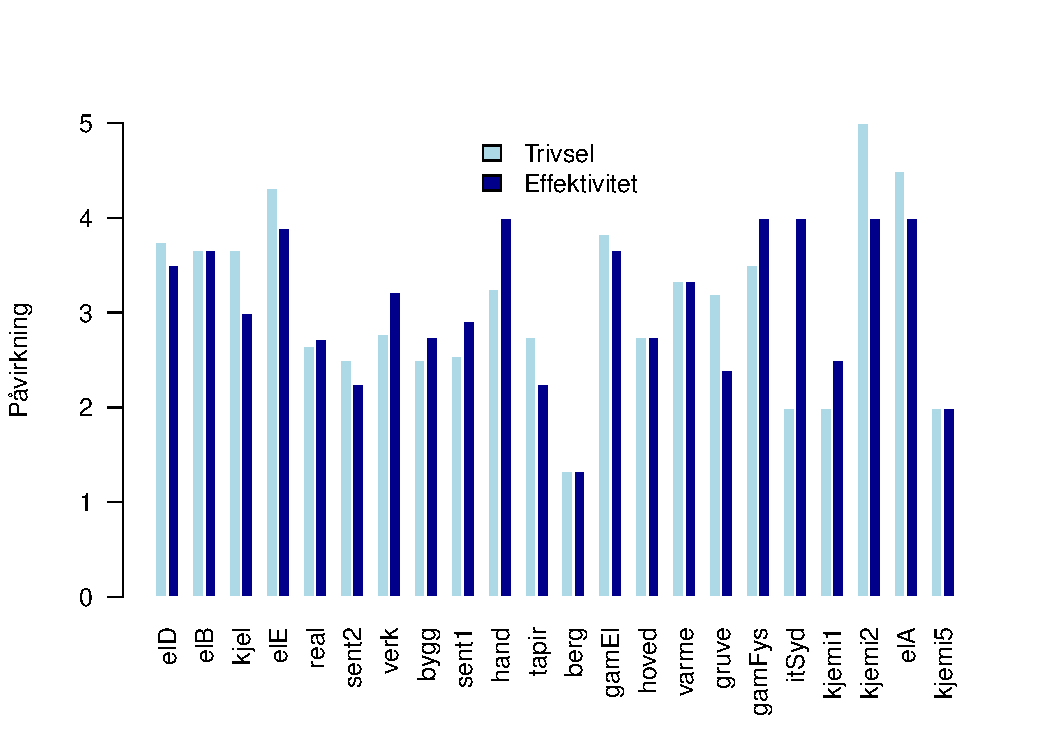
\includegraphics{noiseOnCampus_files/figure-latex/barplotResponses, options-1} \end{center}

\begin{Shaded}
\begin{Highlighting}[]

\NormalTok{mTriv}\OtherTok{=} \FunctionTok{max}\NormalTok{(buildMeans[}\StringTok{\textquotesingle{}trivsel\textquotesingle{}}\NormalTok{,])}
\NormalTok{mEff }\OtherTok{=} \FunctionTok{max}\NormalTok{(buildMeans[}\StringTok{\textquotesingle{}effektivitet\textquotesingle{}}\NormalTok{,])}
\NormalTok{buildMeans[}\StringTok{\textquotesingle{}effektivitet\textquotesingle{}}\NormalTok{,buildMeans[}\StringTok{\textquotesingle{}effektivitet\textquotesingle{}}\NormalTok{,]}\SpecialCharTok{==}\NormalTok{mEff]}
\end{Highlighting}
\end{Shaded}

\begin{verbatim}
##              hand gamFys itSyd kjemi2 elA
## effektivitet    4      4     4      4   4
\end{verbatim}

\begin{Shaded}
\begin{Highlighting}[]
\NormalTok{buildMeans[}\StringTok{\textquotesingle{}trivsel\textquotesingle{}}\NormalTok{,buildMeans[}\StringTok{\textquotesingle{}trivsel\textquotesingle{}}\NormalTok{,]}\SpecialCharTok{==}\NormalTok{mTriv]}
\end{Highlighting}
\end{Shaded}

\begin{verbatim}
## [1] 5
\end{verbatim}

\begin{Shaded}
\begin{Highlighting}[]

\CommentTok{\# sort(buildMeans[\textquotesingle{}trivsel\textquotesingle{},], decreasing = T)}
\end{Highlighting}
\end{Shaded}

\begin{Shaded}
\begin{Highlighting}[]
\FunctionTok{barplot}\NormalTok{(}
\NormalTok{  ((}\FunctionTok{as.matrix}\NormalTok{(buildSd))), }
  \AttributeTok{col =} \FunctionTok{c}\NormalTok{(}\StringTok{"lightblue"}\NormalTok{, }\StringTok{\textquotesingle{}darkblue\textquotesingle{}}\NormalTok{),}
  \AttributeTok{border =} \StringTok{"white"}\NormalTok{,}
  \CommentTok{\# main="Trivsel",}
  \AttributeTok{ylab=}\StringTok{"Standardavvik"}\NormalTok{,}
  \AttributeTok{beside =}\NormalTok{ T,}
  \AttributeTok{las=}\DecValTok{2}\NormalTok{,}
  \CommentTok{\# ylim = c(0,5)}
  \CommentTok{\# space=0.1}
\NormalTok{)}
\FunctionTok{legend}\NormalTok{(}
  \StringTok{"top"}\NormalTok{,}
  \AttributeTok{legend =} \FunctionTok{c}\NormalTok{(}\StringTok{"Trivsel"}\NormalTok{, }\StringTok{"Effektivitet"}\NormalTok{),}
  \AttributeTok{fill =} \FunctionTok{c}\NormalTok{(}\StringTok{"lightblue"}\NormalTok{, }\StringTok{\textquotesingle{}darkblue\textquotesingle{}}\NormalTok{), }\AttributeTok{bty =} \StringTok{\textquotesingle{}n\textquotesingle{}}\NormalTok{)}
\end{Highlighting}
\end{Shaded}

\begin{center}\includegraphics{noiseOnCampus_files/figure-latex/barplotResponseSD, options-1} \end{center}

\begin{Shaded}
\begin{Highlighting}[]
\FunctionTok{pdf}\NormalTok{(}\AttributeTok{file =} \StringTok{\textquotesingle{}./figures/histTrivsel\&EffektivitetSD.pdf\textquotesingle{}}\NormalTok{, }\AttributeTok{width =} \DecValTok{10}\NormalTok{,}\AttributeTok{height =} \DecValTok{6}\NormalTok{)}
\FunctionTok{barplot}\NormalTok{(}
\NormalTok{  ((}\FunctionTok{as.matrix}\NormalTok{(buildSd))), }
  \AttributeTok{col =} \FunctionTok{c}\NormalTok{(}\StringTok{"lightblue"}\NormalTok{, }\StringTok{\textquotesingle{}darkblue\textquotesingle{}}\NormalTok{),}
  \AttributeTok{border =} \StringTok{"white"}\NormalTok{,}
  \CommentTok{\# main="Trivsel",}
  \AttributeTok{ylab=}\StringTok{"Standardavvik"}\NormalTok{,}
  \AttributeTok{beside =}\NormalTok{ T,}
  \AttributeTok{las=}\DecValTok{2}\NormalTok{,}
  \CommentTok{\# ylim = c(0,5)}
  \CommentTok{\# space=0.1}
\NormalTok{)}
\FunctionTok{legend}\NormalTok{(}
  \StringTok{"top"}\NormalTok{,}
  \AttributeTok{legend =} \FunctionTok{c}\NormalTok{(}\StringTok{"Trivsel"}\NormalTok{, }\StringTok{"Effektivitet"}\NormalTok{),}
  \AttributeTok{fill =} \FunctionTok{c}\NormalTok{(}\StringTok{"lightblue"}\NormalTok{, }\StringTok{\textquotesingle{}darkblue\textquotesingle{}}\NormalTok{), }\AttributeTok{bty =} \StringTok{\textquotesingle{}n\textquotesingle{}}\NormalTok{)}
\FunctionTok{dev.off}\NormalTok{()}
\end{Highlighting}
\end{Shaded}

\begin{verbatim}
## pdf 
##   2
\end{verbatim}

\hypertarget{make-building-data}{%
\section{Make building data}\label{make-building-data}}

\begin{Shaded}
\begin{Highlighting}[]
\NormalTok{buildings }\OtherTok{=} \FunctionTok{split}\NormalTok{(d, }\AttributeTok{f =}\NormalTok{ d}\SpecialCharTok{$}\NormalTok{spmHvor)}
\ControlFlowTok{for}\NormalTok{ (build }\ControlFlowTok{in}\NormalTok{ buildings) \{}
    \FunctionTok{print}\NormalTok{(}\FunctionTok{mean}\NormalTok{(build}\SpecialCharTok{$}\NormalTok{spmTriv))}
\NormalTok{\}}
\end{Highlighting}
\end{Shaded}

\begin{verbatim}
## [1] 1.333333
## [1] 2.5
## [1] 4.5
## [1] 3.666667
## [1] 3.75
## [1] 4.315789
## [1] 3.833333
## [1] 3.5
## [1] 3.2
## [1] 3.25
## [1] 2.75
## [1] 2
## [1] 3.666667
## [1] 2
## [1] 5
## [1] 2
## [1] 2.655172
## [1] 2.545455
## [1] 2.5
## [1] 2.75
## [1] 3.333333
## [1] 2.777778
\end{verbatim}

\hypertarget{glmm-fit-on-errytin}{%
\section{GLMM fit on errytin'}\label{glmm-fit-on-errytin}}

\begin{Shaded}
\begin{Highlighting}[]
\FunctionTok{set.seed}\NormalTok{(}\DecValTok{420}\NormalTok{)}
\NormalTok{fitAll }\OtherTok{=} \FunctionTok{glmm}\NormalTok{(spmTriv }\SpecialCharTok{\textasciitilde{}} \DecValTok{0} \SpecialCharTok{+}\NormalTok{ Svartid, }\AttributeTok{varcomps.names =} \FunctionTok{c}\NormalTok{(}\StringTok{""}\NormalTok{), }\AttributeTok{data =}\NormalTok{ d, }\AttributeTok{family.glmm =}\NormalTok{ Gaussian)}
\NormalTok{dSummary }\OtherTok{=} \FunctionTok{summary}\NormalTok{(d)}
\FunctionTok{head}\NormalTok{(d)}
\end{Highlighting}
\end{Shaded}

\hypertarget{glm-fit-on-svartid}{%
\section{GLM fit on Svartid}\label{glm-fit-on-svartid}}

\begin{Shaded}
\begin{Highlighting}[]
\CommentTok{\# Fit}
\NormalTok{fitTidTriv }\OtherTok{=} \FunctionTok{glm}\NormalTok{(}\FunctionTok{factor}\NormalTok{(spmTriv, }\FunctionTok{seq}\NormalTok{(}\DecValTok{1}\NormalTok{, }\DecValTok{5}\NormalTok{, }\DecValTok{1}\NormalTok{)) }\SpecialCharTok{\textasciitilde{}}\NormalTok{ Svartid, }\AttributeTok{data =}\NormalTok{ d, }\AttributeTok{family =} \StringTok{"binomial"}\NormalTok{)}
\NormalTok{fitTidEff }\OtherTok{=} \FunctionTok{glm}\NormalTok{(}\FunctionTok{factor}\NormalTok{(spmEff, }\FunctionTok{seq}\NormalTok{(}\DecValTok{1}\NormalTok{, }\DecValTok{5}\NormalTok{, }\DecValTok{1}\NormalTok{)) }\SpecialCharTok{\textasciitilde{}}\NormalTok{ Svartid, }\AttributeTok{data =}\NormalTok{ d, }\AttributeTok{family =} \StringTok{"binomial"}\NormalTok{)}

\FunctionTok{summary}\NormalTok{(fitTidTriv)}\SpecialCharTok{$}\NormalTok{coefficients}
\end{Highlighting}
\end{Shaded}

\begin{verbatim}
##                  Estimate   Std. Error   z value     Pr(>|z|)
## (Intercept)  1.9382384576 0.2764729103  7.010591 2.373138e-12
## Svartid     -0.0004750205 0.0003684438 -1.289262 1.973071e-01
\end{verbatim}

\begin{Shaded}
\begin{Highlighting}[]
\FunctionTok{summary}\NormalTok{(fitTidEff)}\SpecialCharTok{$}\NormalTok{coefficients}
\end{Highlighting}
\end{Shaded}

\begin{verbatim}
##                  Estimate   Std. Error    z value     Pr(>|z|)
## (Intercept)  1.8286887821 0.2685787185  6.8087628 9.844164e-12
## Svartid     -0.0003192636 0.0003758653 -0.8494097 3.956534e-01
\end{verbatim}

\begin{Shaded}
\begin{Highlighting}[]
\FunctionTok{summary}\NormalTok{(fitTidEff)}
\end{Highlighting}
\end{Shaded}

\begin{verbatim}
## 
## Call:
## glm(formula = factor(spmEff, seq(1, 5, 1)) ~ Svartid, family = "binomial", 
##     data = d)
## 
## Deviance Residuals: 
##     Min       1Q   Median       3Q      Max  
## -1.9809   0.5518   0.5556   0.5606   0.7622  
## 
## Coefficients:
##               Estimate Std. Error z value Pr(>|z|)    
## (Intercept)  1.8286888  0.2685787   6.809 9.84e-12 ***
## Svartid     -0.0003193  0.0003759  -0.849    0.396    
## ---
## Signif. codes:  0 '***' 0.001 '**' 0.01 '*' 0.05 '.' 0.1 ' ' 1
## 
## (Dispersion parameter for binomial family taken to be 1)
## 
##     Null deviance: 112.94  on 133  degrees of freedom
## Residual deviance: 112.30  on 132  degrees of freedom
## AIC: 116.3
## 
## Number of Fisher Scoring iterations: 4
\end{verbatim}

\hypertarget{glm-fit-on-noise-types}{%
\section{GLM fit on noise types}\label{glm-fit-on-noise-types}}

\begin{Shaded}
\begin{Highlighting}[]
\NormalTok{factors }\OtherTok{=} \FunctionTok{c}\NormalTok{(}\StringTok{"spmTriv"}\NormalTok{, }\StringTok{"spmEff"}\NormalTok{, }\StringTok{"byggestoy1"}\NormalTok{, }\StringTok{"personstoy1"}\NormalTok{, }\StringTok{"trafikk1"}\NormalTok{, }\StringTok{"vifte1"}\NormalTok{,}
    \StringTok{"annet1"}\NormalTok{, }\StringTok{"byggestoy2"}\NormalTok{, }\StringTok{"personstoy2"}\NormalTok{, }\StringTok{"trafikk2"}\NormalTok{, }\StringTok{"vifte2"}\NormalTok{, }\StringTok{"annet2"}\NormalTok{)}
\NormalTok{dFactored }\OtherTok{=}\NormalTok{ d}
\CommentTok{\# factorize = function()}
\ControlFlowTok{for}\NormalTok{ (f }\ControlFlowTok{in}\NormalTok{ factors) \{}
\NormalTok{    dFactored[f, ] }\OtherTok{=} \FunctionTok{factor}\NormalTok{(d[f, ], }\FunctionTok{seq}\NormalTok{(}\DecValTok{1}\NormalTok{, }\DecValTok{5}\NormalTok{, }\DecValTok{1}\NormalTok{), }\AttributeTok{ordered =}\NormalTok{ T)}
\NormalTok{\}}

\NormalTok{fitTrivSource }\OtherTok{=} \FunctionTok{glm}\NormalTok{(}\FunctionTok{factor}\NormalTok{(spmTriv, }\FunctionTok{seq}\NormalTok{(}\DecValTok{1}\NormalTok{, }\DecValTok{5}\NormalTok{, }\DecValTok{1}\NormalTok{), }\AttributeTok{ordered =}\NormalTok{ T) }\SpecialCharTok{\textasciitilde{}}\NormalTok{ byggestoy1 }\SpecialCharTok{+}\NormalTok{ personstoy1 }\SpecialCharTok{+}
\NormalTok{    trafikk1 }\SpecialCharTok{+}\NormalTok{ vifte1 }\SpecialCharTok{+}\NormalTok{ annet1, }\AttributeTok{data =}\NormalTok{ dFactored, }\AttributeTok{family =} \StringTok{"binomial"}\NormalTok{)}
\FunctionTok{summary}\NormalTok{(fitTrivSource)}
\end{Highlighting}
\end{Shaded}

\begin{verbatim}
## 
## Call:
## glm(formula = factor(spmTriv, seq(1, 5, 1), ordered = T) ~ byggestoy1 + 
##     personstoy1 + trafikk1 + vifte1 + annet1, family = "binomial", 
##     data = dFactored)
## 
## Deviance Residuals: 
##      Min        1Q    Median        3Q       Max  
## -2.58146   0.00000   0.00004   0.21799   1.78586  
## 
## Coefficients:
##                Estimate Std. Error z value Pr(>|z|)   
## (Intercept)  -1.310e+00  7.180e-01  -1.824  0.06808 . 
## byggestoy12  -5.326e-01  9.382e-01  -0.568  0.57021   
## byggestoy13   2.046e+00  1.356e+00   1.509  0.13119   
## byggestoy14   1.879e+01  5.093e+03   0.004  0.99706   
## byggestoy15   3.307e+00  1.228e+00   2.694  0.00707 **
## personstoy12  2.050e+00  9.444e-01   2.171  0.02993 * 
## personstoy13  1.704e+00  9.764e-01   1.745  0.08103 . 
## personstoy14  3.424e+00  1.359e+00   2.520  0.01174 * 
## personstoy15  2.111e+01  6.189e+03   0.003  0.99728   
## trafikk12    -1.124e+00  1.643e+00  -0.684  0.49402   
## trafikk13     6.090e+00  1.063e+05   0.000  0.99995   
## trafikk14     2.228e+01  1.612e+04   0.001  0.99890   
## trafikk15    -3.049e+01  1.108e+05   0.000  0.99978   
## vifte12      -5.778e-02  9.986e-01  -0.058  0.95386   
## vifte13       1.815e+01  5.972e+03   0.003  0.99758   
## vifte14       1.673e+01  8.444e+03   0.002  0.99842   
## vifte15       2.065e+01  9.031e+03   0.002  0.99818   
## annet12       2.058e+01  4.893e+03   0.004  0.99664   
## annet13       7.770e-01  1.759e+00   0.442  0.65876   
## annet14      -1.713e+01  2.172e+04  -0.001  0.99937   
## annet15       1.080e+01  1.067e+05   0.000  0.99992   
## ---
## Signif. codes:  0 '***' 0.001 '**' 0.01 '*' 0.05 '.' 0.1 ' ' 1
## 
## (Dispersion parameter for binomial family taken to be 1)
## 
##     Null deviance: 109.398  on 133  degrees of freedom
## Residual deviance:  52.957  on 113  degrees of freedom
##   (12 observations deleted due to missingness)
## AIC: 94.957
## 
## Number of Fisher Scoring iterations: 20
\end{verbatim}

\begin{Shaded}
\begin{Highlighting}[]
\FunctionTok{cov}\NormalTok{(d}\SpecialCharTok{$}\NormalTok{spmTriv, d}\SpecialCharTok{$}\NormalTok{byggestoy1)}
\end{Highlighting}
\end{Shaded}

\begin{verbatim}
## [1] 1.035911
\end{verbatim}

\begin{Shaded}
\begin{Highlighting}[]
\FunctionTok{cov}\NormalTok{(d}\SpecialCharTok{$}\NormalTok{spmEff, d}\SpecialCharTok{$}\NormalTok{byggestoy2)}
\end{Highlighting}
\end{Shaded}

\begin{verbatim}
## [1] 1.2112
\end{verbatim}

\begin{Shaded}
\begin{Highlighting}[]
\FunctionTok{par}\NormalTok{(d)}
\end{Highlighting}
\end{Shaded}

\hypertarget{initial-data-observations}{%
\section{Initial data observations}\label{initial-data-observations}}

\begin{Shaded}
\begin{Highlighting}[]
\FunctionTok{hist}\NormalTok{(d}\SpecialCharTok{$}\NormalTok{spmTriv, }\AttributeTok{breaks =} \FunctionTok{seq}\NormalTok{(}\FloatTok{0.5}\NormalTok{, }\FloatTok{5.5}\NormalTok{, }\DecValTok{1}\NormalTok{), }\AttributeTok{freq =}\NormalTok{ T)}
\FunctionTok{lines}\NormalTok{(}\FunctionTok{density}\NormalTok{(d}\SpecialCharTok{$}\NormalTok{spmTriv, }\AttributeTok{bw =} \DecValTok{1}\NormalTok{, }\AttributeTok{from =} \DecValTok{1}\NormalTok{, }\AttributeTok{to =} \DecValTok{5}\NormalTok{))}
\end{Highlighting}
\end{Shaded}

\begin{center}\includegraphics{noiseOnCampus_files/figure-latex/initial, options-1} \end{center}

\begin{Shaded}
\begin{Highlighting}[]
\FunctionTok{hist}\NormalTok{(d}\SpecialCharTok{$}\NormalTok{spmEff, }\AttributeTok{breaks =} \FunctionTok{seq}\NormalTok{(}\FloatTok{0.5}\NormalTok{, }\FloatTok{5.5}\NormalTok{, }\DecValTok{1}\NormalTok{), }\AttributeTok{freq =}\NormalTok{ T)}
\FunctionTok{lines}\NormalTok{(}\FunctionTok{density}\NormalTok{(d}\SpecialCharTok{$}\NormalTok{spmEff, }\AttributeTok{bw =} \DecValTok{1}\NormalTok{, }\AttributeTok{from =} \DecValTok{1}\NormalTok{, }\AttributeTok{to =} \DecValTok{5}\NormalTok{))}
\end{Highlighting}
\end{Shaded}

\begin{center}\includegraphics{noiseOnCampus_files/figure-latex/initial, options-2} \end{center}

\hypertarget{linear-models}{%
\section{Linear models}\label{linear-models}}

\begin{Shaded}
\begin{Highlighting}[]
\NormalTok{lmTrivSource }\OtherTok{=} \FunctionTok{lm}\NormalTok{(spmTriv }\SpecialCharTok{\textasciitilde{}} \SpecialCharTok{{-}}\DecValTok{1} \SpecialCharTok{+}\NormalTok{ byggestoy1 }\SpecialCharTok{+}\NormalTok{ personstoy1 }\SpecialCharTok{+}\NormalTok{ trafikk1 }\SpecialCharTok{+}\NormalTok{ vifte1 }\SpecialCharTok{+}\NormalTok{ annet1,}
    \AttributeTok{data =}\NormalTok{ d)}
\FunctionTok{summary}\NormalTok{(lmTrivSource)}
\end{Highlighting}
\end{Shaded}

\begin{verbatim}
## 
## Call:
## lm(formula = spmTriv ~ -1 + byggestoy1 + personstoy1 + trafikk1 + 
##     vifte1 + annet1, data = d)
## 
## Residuals:
##     Min      1Q  Median      3Q     Max 
## -3.3250 -0.5627 -0.0132  0.5948  3.8080 
## 
## Coefficients:
##             Estimate Std. Error t value Pr(>|t|)    
## byggestoy1   0.45379    0.04919   9.226 4.35e-16 ***
## personstoy1  0.43678    0.05741   7.608 3.92e-12 ***
## trafikk1    -0.10048    0.13560  -0.741  0.45994    
## vifte1       0.25892    0.08053   3.215  0.00162 ** 
## annet1       0.14296    0.09381   1.524  0.12982    
## ---
## Signif. codes:  0 '***' 0.001 '**' 0.01 '*' 0.05 '.' 0.1 ' ' 1
## 
## Residual standard error: 1.041 on 138 degrees of freedom
## Multiple R-squared:  0.9115, Adjusted R-squared:  0.9083 
## F-statistic: 284.4 on 5 and 138 DF,  p-value: < 2.2e-16
\end{verbatim}

\begin{Shaded}
\begin{Highlighting}[]
\CommentTok{\# pairs(d[,apply(d[1,],2, FUN=is.numeric)])}
\end{Highlighting}
\end{Shaded}

\begin{Shaded}
\begin{Highlighting}[]
\NormalTok{dNumeric }\OtherTok{=} \FunctionTok{select\_if}\NormalTok{(d, is.numeric)}
\FunctionTok{head}\NormalTok{(dNumeric[, }\DecValTok{2}\SpecialCharTok{:}\DecValTok{7}\NormalTok{])}
\end{Highlighting}
\end{Shaded}

\begin{verbatim}
##   spmTriv byggestoy1 personstoy1 trafikk1 vifte1 annet1
## 1       4          4           2        1      2      5
## 2       3          4           1        1      3      1
## 3       1          1           2        1      1      1
## 4       3          1           2        1      1      1
## 5       4          5           2        1      1      1
## 6       3          1           4        1      3      1
\end{verbatim}

\begin{Shaded}
\begin{Highlighting}[]
\NormalTok{lmTrivSource }\OtherTok{=} \FunctionTok{lm}\NormalTok{(spmTriv }\SpecialCharTok{\textasciitilde{}}\NormalTok{ ., }\AttributeTok{data =}\NormalTok{ dNumeric[}\DecValTok{2}\SpecialCharTok{:}\DecValTok{7}\NormalTok{])}
\NormalTok{lmTrivCoefs }\OtherTok{=} \FunctionTok{summary}\NormalTok{(lmTrivSource)}\SpecialCharTok{$}\NormalTok{coefficients}
\NormalTok{lmTIntercept }\OtherTok{=}\NormalTok{ lmTrivCoefs[}\StringTok{"(Intercept)"}\NormalTok{, }\StringTok{"Estimate"}\NormalTok{]}
\NormalTok{lmTBygg }\OtherTok{=}\NormalTok{ lmTrivCoefs[}\StringTok{"byggestoy1"}\NormalTok{, }\StringTok{"Estimate"}\NormalTok{]}
\NormalTok{lmTPers }\OtherTok{=}\NormalTok{ lmTrivCoefs[}\StringTok{"personstoy1"}\NormalTok{, }\StringTok{"Estimate"}\NormalTok{]}
\NormalTok{lmTVift }\OtherTok{=}\NormalTok{ lmTrivCoefs[}\StringTok{"vifte1"}\NormalTok{, }\StringTok{"Estimate"}\NormalTok{]}
\NormalTok{yEst }\OtherTok{=}\NormalTok{ lmTBygg }\SpecialCharTok{*}\NormalTok{ (}\DecValTok{1}\SpecialCharTok{:}\DecValTok{5}\NormalTok{) }\SpecialCharTok{+}\NormalTok{ lmTPers }\SpecialCharTok{*}\NormalTok{ (}\DecValTok{1}\SpecialCharTok{:}\DecValTok{5}\NormalTok{) }\SpecialCharTok{+}\NormalTok{ lmTVift }\SpecialCharTok{*}\NormalTok{ (}\DecValTok{1}\SpecialCharTok{:}\DecValTok{5}\NormalTok{)}
\FunctionTok{plot}\NormalTok{(dNumeric[, }\StringTok{"byggestoy1"}\NormalTok{], dNumeric[, }\StringTok{"spmTriv"}\NormalTok{], )}
\end{Highlighting}
\end{Shaded}

\begin{center}\includegraphics{noiseOnCampus_files/figure-latex/numericVals, options-1} \end{center}

\begin{Shaded}
\begin{Highlighting}[]
\FunctionTok{plot}\NormalTok{(yEst)}
\end{Highlighting}
\end{Shaded}

\begin{center}\includegraphics{noiseOnCampus_files/figure-latex/numericVals, options-2} \end{center}

\begin{Shaded}
\begin{Highlighting}[]
\FunctionTok{pairs}\NormalTok{(dNumeric[, }\DecValTok{2}\SpecialCharTok{:}\DecValTok{7}\NormalTok{])}
\end{Highlighting}
\end{Shaded}

\begin{center}\includegraphics{noiseOnCampus_files/figure-latex/pairs, options-1} \end{center}

\begin{Shaded}
\begin{Highlighting}[]
\FunctionTok{library}\NormalTok{(GGally)}
\FunctionTok{ggpairs}\NormalTok{(dNumeric[, }\DecValTok{2}\SpecialCharTok{:}\DecValTok{7}\NormalTok{])}
\end{Highlighting}
\end{Shaded}

\begin{center}\includegraphics{noiseOnCampus_files/figure-latex/pairs, options-2} \end{center}

\begin{Shaded}
\begin{Highlighting}[]
\FunctionTok{ggpairs}\NormalTok{(dNumeric[, }\DecValTok{8}\SpecialCharTok{:}\DecValTok{13}\NormalTok{])}
\end{Highlighting}
\end{Shaded}

\begin{center}\includegraphics{noiseOnCampus_files/figure-latex/pairs, options-3} \end{center}

\hypertarget{building-relations}{%
\section{Building relations}\label{building-relations}}

\hypertarget{anc-and-noise-type-correlation}{%
\section{ANC and noise type correlation}\label{anc-and-noise-type-correlation}}

How to do this?
Initially we will look at noise types and how much they disturb when the individual uses ANC compared to when the individual is not.

\begin{Shaded}
\begin{Highlighting}[]
\NormalTok{ntTriv }\OtherTok{=} \FunctionTok{colnames}\NormalTok{(d)[}\DecValTok{7}\SpecialCharTok{:}\DecValTok{11}\NormalTok{]}
\NormalTok{ntEff }\OtherTok{=} \FunctionTok{colnames}\NormalTok{(d)[}\DecValTok{13}\SpecialCharTok{:}\DecValTok{17}\NormalTok{]}
\NormalTok{ntColnames }\OtherTok{=} \FunctionTok{c}\NormalTok{(}
  \StringTok{\textquotesingle{}Konstruksjon\textquotesingle{}}\NormalTok{, }\StringTok{\textquotesingle{}Person\textquotesingle{}}\NormalTok{, }\StringTok{\textquotesingle{}Trafikk\textquotesingle{}}\NormalTok{, }\StringTok{\textquotesingle{}Vifte\textquotesingle{}}\NormalTok{, }\StringTok{\textquotesingle{}Annet\textquotesingle{}}\NormalTok{)}
\NormalTok{ntRownames }\OtherTok{=} \FunctionTok{c}\NormalTok{(}
  \StringTok{\textquotesingle{}Trivsel m/ ANC\textquotesingle{}}\NormalTok{, }\StringTok{\textquotesingle{}Trivsel u/ ANC\textquotesingle{}}\NormalTok{, }\StringTok{\textquotesingle{}Effektivitet m/ ANC\textquotesingle{}}\NormalTok{,}
  \StringTok{\textquotesingle{}Effektivitet u/ ANC\textquotesingle{}}\NormalTok{)}
\NormalTok{ntAnc }\OtherTok{=} \FunctionTok{data.frame}\NormalTok{(}
  \FunctionTok{matrix}\NormalTok{(}
    \AttributeTok{ncol =} \FunctionTok{length}\NormalTok{(ntTriv), }\AttributeTok{nrow =} \DecValTok{4}\NormalTok{,}
    \AttributeTok{dimnames=}\FunctionTok{list}\NormalTok{(ntRownames, ntColnames)}
\NormalTok{  )}
\NormalTok{)}

\CommentTok{\# Find mean noise type disturbances}
\NormalTok{ancBool }\OtherTok{=}\NormalTok{ d[,}\StringTok{"spmTiltak\_1"}\NormalTok{] }\SpecialCharTok{==} \StringTok{"mNc"}
\NormalTok{ntAnc[ntColnames] }\OtherTok{=} \FunctionTok{c}\NormalTok{(}
  \FunctionTok{apply}\NormalTok{(d[ancBool, ntTriv], }\AttributeTok{FUN =}\NormalTok{ mean, }\AttributeTok{MARGIN =} \DecValTok{2}\NormalTok{),}
  \FunctionTok{apply}\NormalTok{(d[}\SpecialCharTok{!}\NormalTok{ancBool, ntTriv], }\AttributeTok{FUN =}\NormalTok{ mean, }\AttributeTok{MARGIN =} \DecValTok{2}\NormalTok{),}
  \FunctionTok{apply}\NormalTok{(d[ancBool,ntEff], }\AttributeTok{FUN =}\NormalTok{ mean, }\AttributeTok{MARGIN =} \DecValTok{2}\NormalTok{),}
  \FunctionTok{apply}\NormalTok{(d[}\SpecialCharTok{!}\NormalTok{ancBool,ntEff], }\AttributeTok{FUN =}\NormalTok{ mean, }\AttributeTok{MARGIN =} \DecValTok{2}\NormalTok{)}
\NormalTok{)}

\CommentTok{\# Barplot}
\NormalTok{reOrder }\OtherTok{=} \FunctionTok{c}\NormalTok{(}\DecValTok{1}\NormalTok{,}\DecValTok{3}\NormalTok{,}\DecValTok{2}\NormalTok{,}\DecValTok{4}\NormalTok{)}
\NormalTok{cols }\OtherTok{=} \FunctionTok{c}\NormalTok{(}\StringTok{"\#b1fbf5"}\NormalTok{, }\StringTok{\textquotesingle{}\#d5a7fb\textquotesingle{}}\NormalTok{, }\StringTok{\textquotesingle{}\#59f7ea\textquotesingle{}}\NormalTok{, }\StringTok{\textquotesingle{}\#be77f9\textquotesingle{}}\NormalTok{)}
\FunctionTok{barplot}\NormalTok{(}
\NormalTok{  ((}\FunctionTok{as.matrix}\NormalTok{(ntAnc[reOrder,]))), }
  \AttributeTok{col =}\NormalTok{ cols[reOrder],}
  \AttributeTok{border =} \StringTok{"white"}\NormalTok{,}
  \CommentTok{\# main="Trivsel",}
  \AttributeTok{ylab=}\StringTok{"P\textbackslash{}u00E5virkning"}\NormalTok{,}
  \AttributeTok{beside =}\NormalTok{ T,}
  \CommentTok{\# las=2,}
  \AttributeTok{ylim =} \FunctionTok{c}\NormalTok{(}\DecValTok{0}\NormalTok{,}\DecValTok{5}\NormalTok{)}
  \CommentTok{\# space=0.1}
\NormalTok{)}
\FunctionTok{legend}\NormalTok{(}
  \StringTok{"top"}\NormalTok{,}
  \AttributeTok{legend =}\NormalTok{ ntRownames[reOrder],}
  \AttributeTok{fill =}\NormalTok{ cols[reOrder], }\AttributeTok{bty =} \StringTok{\textquotesingle{}n\textquotesingle{}}\NormalTok{)}
\end{Highlighting}
\end{Shaded}

\begin{center}\includegraphics{noiseOnCampus_files/figure-latex/ANCNoisetype, options-1} \end{center}

\end{document}
